\hypertarget{_d_s_std_8h}{
\section{DSStd.h File Reference}
\label{_d_s_std_8h}\index{DSStd.h@{DSStd.h}}
}


Header file for the design space toolbox.  


{\ttfamily \#include $<$stdio.h$>$}\par
{\ttfamily \#include $<$stdlib.h$>$}\par
{\ttfamily \#include \char`\"{}DSTypes.h\char`\"{}}\par
{\ttfamily \#include \char`\"{}DSIO.h\char`\"{}}\par
{\ttfamily \#include \char`\"{}DSErrors.h\char`\"{}}\par
{\ttfamily \#include \char`\"{}DSMemoryManager.h\char`\"{}}\par
{\ttfamily \#include \char`\"{}DSVariable.h\char`\"{}}\par
{\ttfamily \#include \char`\"{}DSMatrix.h\char`\"{}}\par
{\ttfamily \#include \char`\"{}DSMatrixArray.h\char`\"{}}\par
Include dependency graph for DSStd.h:\nopagebreak
\begin{figure}[H]
\begin{center}
\leavevmode
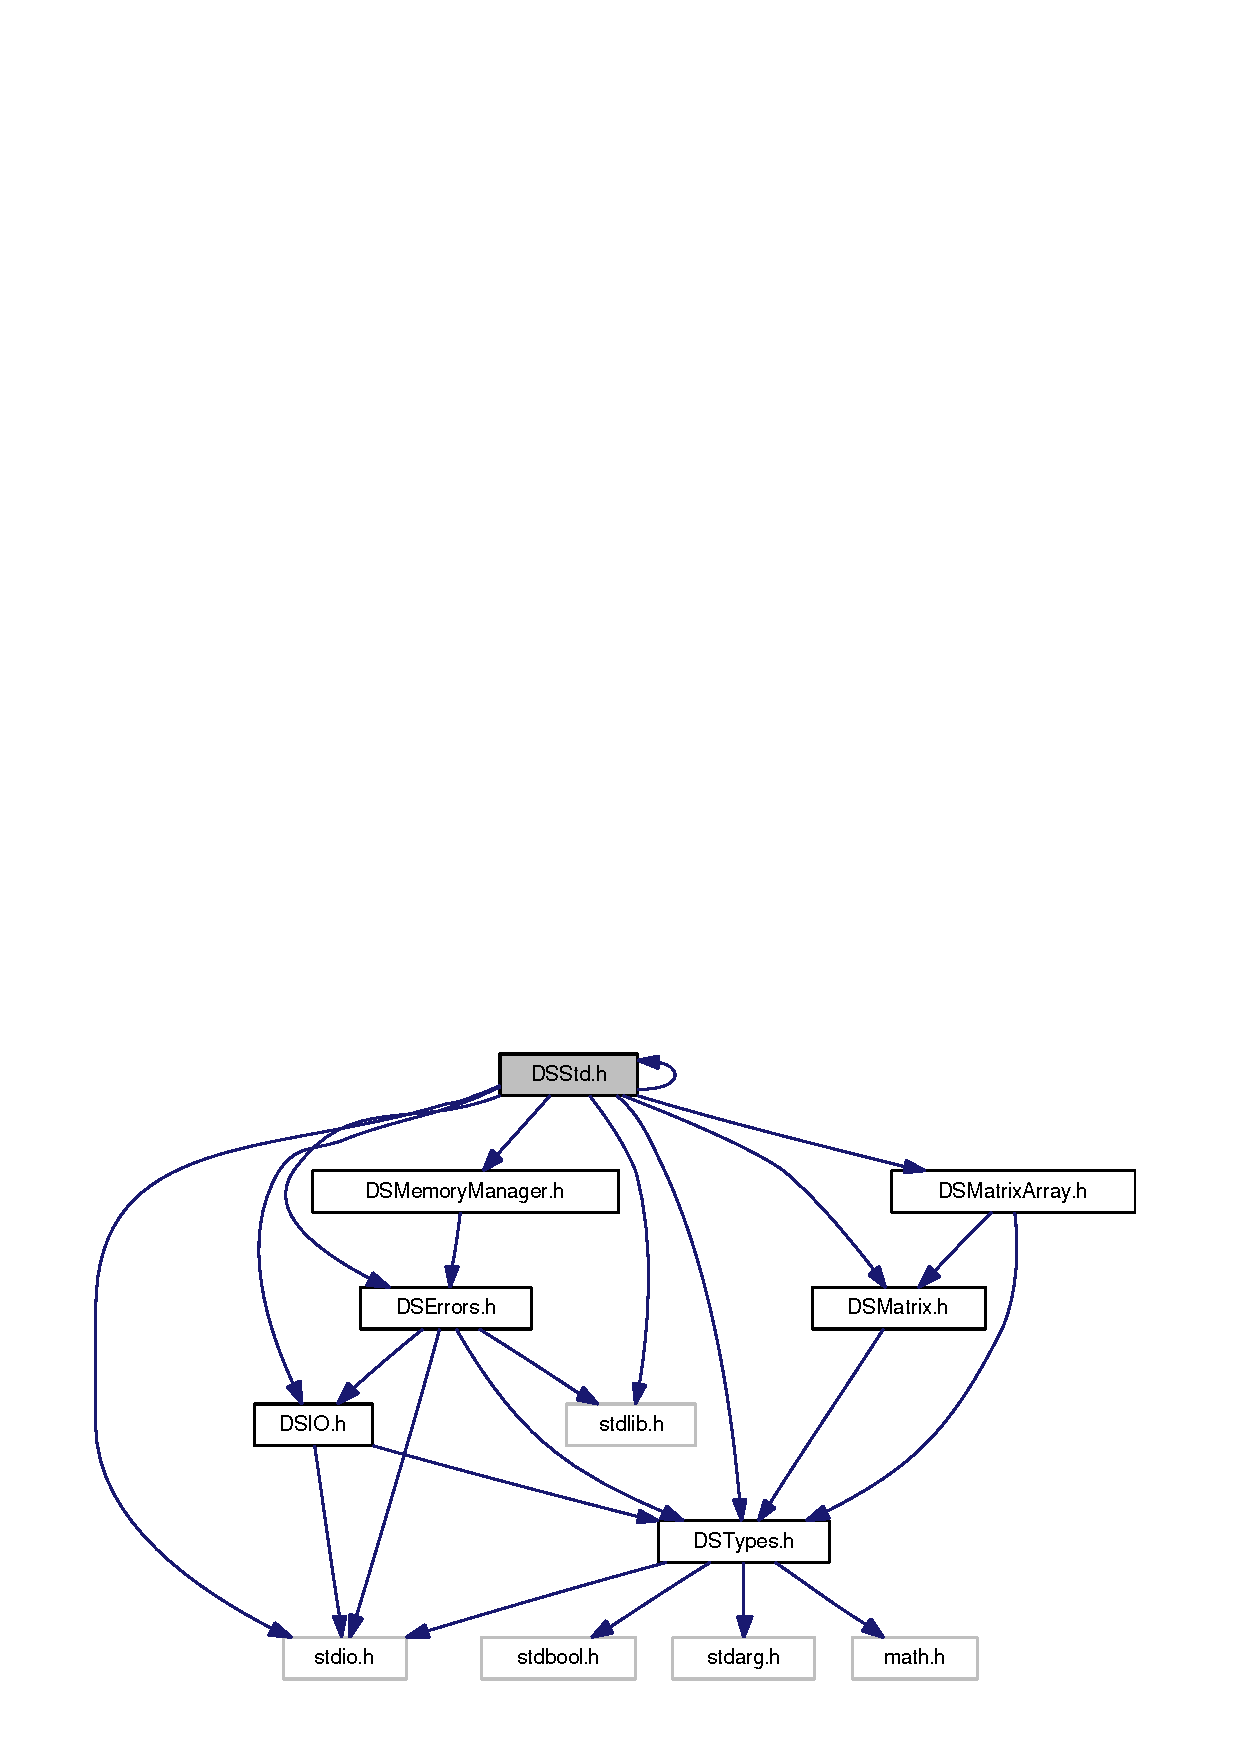
\includegraphics[width=272pt]{_d_s_std_8h__incl}
\end{center}
\end{figure}
This graph shows which files directly or indirectly include this file:\nopagebreak
\begin{figure}[H]
\begin{center}
\leavevmode

\includegraphics[width=60pt]{_d_s_std_8h__dep__incl}
\end{center}
\end{figure}


\subsection{Detailed Description}
Header file for the design space toolbox. Copyright (C) 2011 Jason Lomnitz.\par
\par


This file is part of the Design Space Toolbox V2 (C Library).

The Design Space Toolbox V2 is free software: you can redistribute it and/or modify it under the terms of the GNU General Public License as published by the Free Software Foundation, either version 3 of the License, or (at your option) any later version.

The Design Space Toolbox V2 is distributed in the hope that it will be useful, but WITHOUT ANY WARRANTY; without even the implied warranty of MERCHANTABILITY or FITNESS FOR A PARTICULAR PURPOSE. See the GNU General Public License for more details.

You should have received a copy of the GNU General Public License along with the Design Space Toolbox. If not, see $<$\href{http://www.gnu.org/licenses/}{\tt http://www.gnu.org/licenses/}$>$.

\begin{DoxyAuthor}{Author}
Jason Lomnitz. 
\end{DoxyAuthor}
\begin{DoxyDate}{Date}
2011
\end{DoxyDate}
\begin{Desc}
\item[\hyperlink{todo__todo000002}{Todo}]Add all previous functionality. 

Add vertex enumeration functionality.\end{Desc}
